\documentclass[conference]{IEEEtran}
\IEEEoverridecommandlockouts
% The preceding line is only needed to identify funding in the first footnote. If that is unneeded, please comment it out.
\usepackage{cite}
\usepackage{amsmath,amssymb,amsfonts}
\usepackage{algorithmic}
\usepackage{graphicx}
\usepackage{textcomp}
\usepackage{hyperref}
\usepackage{xcolor}
\def\BibTeX{{\rm B\kern-.05em{\sc i\kern-.025em b}\kern-.08em
    T\kern-.1667em\lower.7ex\hbox{E}\kern-.125emX}}
\begin{document}

\title{On Board Electrical Vehicle Charger}
\author{
\IEEEauthorblockN{Sanket Shyamsunder Sarmalkar}
\IEEEauthorblockA{\textit{Department of Electrical and Electronics Engineering} \\
\textit{National Institute of Technology Goa}\\
Cuncolim, Goa 403701, India \\
sanketsarmalkar@nitgoa.ac.in}
\and
\IEEEauthorblockN{Rathod Mehulkumar Pratap}
\IEEEauthorblockA{\textit{Department of Electrical and Electronics Engineering} \\
\textit{National Institute of Technology Goa}\\
Cuncolim, Goa 403701, India \\
rathodmehulkumarpratap@nitgoa.ac.in}
\and
\IEEEauthorblockN{Dr. Soumitra Das}
\IEEEauthorblockA{\textit{Department of Electrical and Electronics Engineering} \\
\textit{National Institute of Technology Goa}\\
Cuncolim, Goa 403701, India \\
sdas@nitgoa.ac.in}
}


\maketitle

\begin{abstract}
The rise of second-generation hybrid and Electric Vehicles spearheads the automotive industry's shift away from traditional fossil fuel vehicles. Vital to these electric systems is the Battery Management System (BMS), crucial in EVs and renewable energy storage. This project delves into BMS technologies, emphasizing state of charge (SOC) estimation via Extended Kalman Filter, battery charging techniques, and converter topology. It addresses monitoring, balancing, and protection functions, alongside voltage and current management. Discussions encompass cell balancing circuits, control reliability, and efficiency, scrutinizing advantages and drawbacks.
\end{abstract}

\begin{IEEEkeywords}
charging method, method, lithium-ion(Li-ion) battery, CCCV method, SOC estimation, extended kalman filter.
\end{IEEEkeywords}

\section{Introduction}
The depletion of fossil fuels and their adverse effects on ecosystems emphasize the urgent need for transitioning to renewable energy sources and alternative transportation technologies. The excessive extraction and utilization of fossil fuels lead to significant CO2 and greenhouse gas emissions (GHGE). Transitioning to renewable energy sources and electrifying transportation, particularly with Electric Vehicles (EVs) and Hybrid Electric Vehicles (HEVs), is essential. However, the intermittent nature of renewables presents challenges to maintaining a consistent power supply. Energy Storage Systems (ESSs) address this by storing surplus energy during peak production and releasing it when demand is high or renewable generation is low.

EVs and HEVs utilize batteries for power, offering high energy density, low environmental impact, and durable performance. Advancements in battery technology are crucial for wider EV adoption, focusing on enhancing storage capacity, reducing charging times, and lowering costs. Lithium-ion (Li-ion) batteries are prevalent in EVs due to their favorable characteristics, although research explores other chemistries.

Li-ion batteries offer improved reliability, power density, energy density, and efficiency. However, they require careful management to prevent safety hazards and aging. State of Charge (SoC) estimation is critical, considering the battery's high non-linearity and time-varying characteristics. SoC estimation, often done through sophisticated algorithms like Extended Kalman Filters, ensures safe and efficient battery operation.

Despite their advantages, HEVs face drawbacks such as high costs, limited range and speed, and lengthy charging times. Li-ion batteries, constituting a significant portion of HEV costs, also necessitate infrastructure development for charging stations. Charging schemes significantly impact battery life, efficiency, and charging times, underscoring the importance of robust charger design.

In summary, the transition to renewable energy and electrified transportation is imperative. Li-ion batteries play a crucial role in this transition, requiring precise SoC estimation for safe and efficient operation. Overcoming HEV drawbacks demands innovations in battery technology and charging infrastructure.

\section{Literature Survey}

\subsection{Charging Schemes}
\hspace{0.5cm}Various charging schemes for batteries are present in the 
literature and practice. Details of some main charging 
schemes are presented in this section. 
\subsubsection{Constant Voltage Charging Scheme (CV) }
\begin{itemize}
    \item \textbf{Description}:
    \begin{itemize}
        \item The battery is charged using a DC power supply until it reaches the set-point voltage.
        \item Li-ion cells typically have a nominal set-point voltage of 4.2 volts with a tolerance of +/- 50 millivolts.
        \item The maximum allowable charging current is 1C.
    \end{itemize}
    
    \item \textbf{Preference for Pb-acid Batteries}:
    \begin{itemize}
        \item This charging method is preferred for Pb-acid batteries because each individual cell equalizes the charge among them.
    \end{itemize}
    
    \item \textbf{Drawbacks}:
    \begin{itemize}
        \item The battery may not reach full charge using this method.
        \item Charging time exceeds 2 hours, making it relatively slow.
    \end{itemize}
\end{itemize}
\subsubsection{Constant Current Charging Scheme (CC) }
\begin{itemize}
    \item \textbf{Description:}
    \begin{itemize}
        \item Battery is charged with a uniformly constant current.
        \item Not preferred for batteries with more cells as some cells may become fully charged before others.
        \item Leads to inefficiency and over-stress on cells.
    \end{itemize}
        
    \item \textbf{Effects of Higher Charging Currents}:
    \begin{itemize}
        \item Higher charging currents decrease charging efficiency due to joule heating.
        \item Joule heating, also known as ohmic or resistive heating, occurs due to electric current flow through the battery's internal resistance.
    \end{itemize}
    
    \item \textbf{Limitations of Fast Charging}:
    \begin{itemize}
        \item Fast charging is not feasible due to these reasons associated with this charging scheme.
    \end{itemize}
    
    \item \textbf{Drawbacks}:
    \begin{itemize}
        \item Maintaining low charge current increases charging time.
        \item Implementing fast charging for Li-ion batteries requires higher charging current.
    \end{itemize}
\end{itemize}

\subsubsection{Constant Current Constant Voltage Charging Scheme (CC CV) }
\begin{itemize}
    \item \textbf{Procedure:}
    \begin{itemize}
        \item \textbf{Pre-charge Mode}:
        \begin{itemize}
            \item Deeply discharged cells (voltage below 3V) are charged with 10% of full charge current.
            \item Prevents overheating of cells until they can accept full charge current.
        \end{itemize}
        
        \item \textbf{Constant Current Mode}:
        \begin{itemize}
            \item Battery charged below 1C rate until it reaches 4.2V.
            \item Higher charging current rates lead to rapid voltage rise, shortening constant current stage without reducing overall charging time.
        \end{itemize}
        
        \item \textbf{Constant Voltage Mode}:
        \begin{itemize}
            \item Battery charged at constant voltage of 4.2V.
            \item Constant current mode not extended to 100% State of Charge (SoC) to avoid overheating and stress on cells.
            \item Battery not fully charged at 4.2V; further charging required in constant voltage mode.
            \item Current drops to 0.1C as charging nears termination.
        \end{itemize}
        
        \item \textbf{Charge Termination Mode}:
        \begin{itemize}
            \item Charge termination achieved via minimum charge current method or timer method.
            \item In minimum current method, charge current monitored; termination occurs as it reaches 0.02C - 0.07C.
        \end{itemize}
    \end{itemize}
    
    \item \textbf{Drawback}:
    \begin{itemize}
        \item Despite advantages, conventional charging takes a long time (at least more than 2 hours) to completely charge the battery.
    \end{itemize}
\end{itemize}

\subsection{Converter Topology: }
\subsubsection{Buck Converter Topology:}
\begin{itemize}
  \item Simplicity, high efficiency, and voltage step-down capability make it popular in DC-DC conversion applications.
  \item Widely utilized in energy storage systems and power supplies for size, cost, and efficiency optimization.
  \item Advantages include high efficiency, simplicity, and cost-effectiveness.
\end{itemize}

\subsubsection{Three-Phase Rectifiers:}
\begin{itemize}
  \item Prevalent in grid-connected systems for converting AC power to DC efficiently.
  \item Suitable for converting three-phase AC power from renewable sources (e.g., wind turbines, solar arrays) into DC.
  \item Appreciated for robustness, reduced harmonic distortion, and compatibility with grid-tied systems.
\end{itemize}

These technologies play crucial roles in advancing battery management, charging methodologies, and power conversion techniques in renewable energy systems and electric vehicles. Ongoing research aims to enhance efficiency, safety, and adaptability across diverse applications.

\subsection{SOC Estimation :}
\hspace{0.5cm}Comparing SoC estimation methods like the Extended Kalman Filter (EKF), Coulomb Counting, and Voltage-Based Methods reveals trade-offs in accuracy, complexity, and computational demands.
The EKF, adept with nonlinear battery models, offers precise estimations with uncertainty metrics. However, it demands careful parameter tuning and has higher computational needs.
Coulomb Counting, simple and computationally light, integrates current over time for SoC estimation. Yet, it's prone to cumulative errors and struggles with nonlinear battery behavior.
Voltage-Based Methods, though easy to implement and fast, can suffer from accuracy degradation due to battery aging and temperature changes. They're often tailored to specific chemistries, limiting their broad applicability.
The choice hinges on application requirements, with EKF offering accuracy at the cost of complexity, Coulomb Counting favoring simplicity over precision, and Voltage-Based Methods offering quick estimates with some accuracy compromises.
\subsubsection{Battery Equivalent Circuit Model :}
Battery design typically involves modeling the battery using electrical circuit representations to understand its behavior and performance characteristics. One common approach is to use an equivalent circuit model (ECM) to represent the electrochemical processes within the battery. Here's an overview:
\begin{itemize}
  \item \textbf{Internal Resistance ($R_0$):} Represents the internal losses within the battery, including resistance from electrolyte, electrodes, and current collectors.
  
  \item \textbf{Resistance-Capacitance (RC) Network:}
  \begin{itemize}
    \item $R_1$ and $R_2$: Represent the resistive losses associated with the charge transfer process at the electrodes.
    \item $C_1$ and $C_2$: Represent the capacitive behavior due to the diffusion processes within the electrodes.
  \end{itemize}
  
  \item \textbf{Open Circuit Voltage (OCV):} Represents the voltage of the battery when no current is flowing. It is typically voltage-dependent on the state of charge (SOC) and temperature.
  
  \item \textbf{Terminal Voltage ($V_t$):} The actual voltage output of the battery terminals, which is affected by the internal resistance, voltage drop across the resistances, and the open circuit voltage.
\end{itemize}


\section{Circuit Diagram :}

\section{Simulation :}
\hspace{0.5cm}The Simulation Circuit for the CCCV mode of battery in this case LG 18650HG2 (3.0Ah) Battery is shown in fig. \ref{Main_Simulink_Circuit}.
\subsection{Simulink :}
\begin{figure}[htbp]
    \centering
    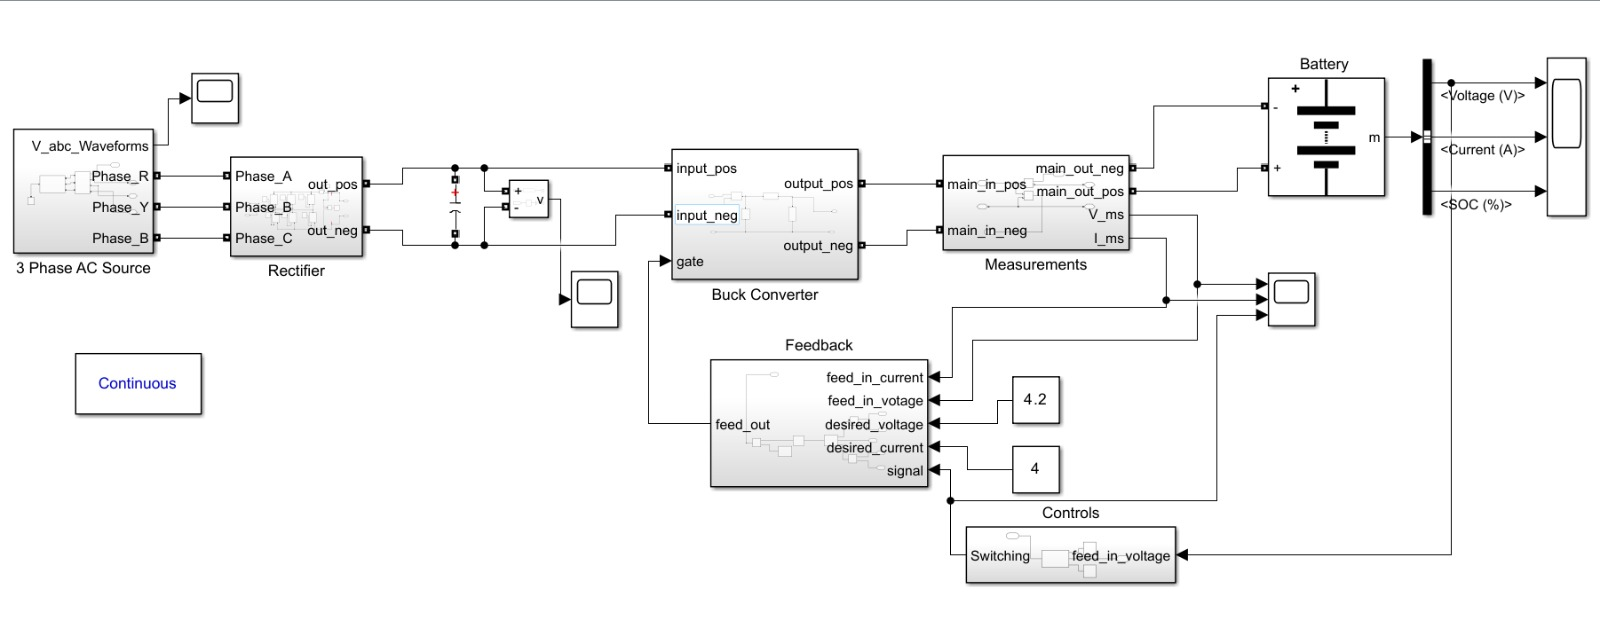
\includegraphics[width=0.5\textwidth]{images/main_simu.jpeg}
    \caption{Main Circuit}
    \label{Main_Simulink_Circuit}
\end{figure}

The very First block after the source is the Three Phase Rectifier Circuit shown in fig. \ref{rectifier_circuit}.
\begin{figure}[htbp]
    \centering
    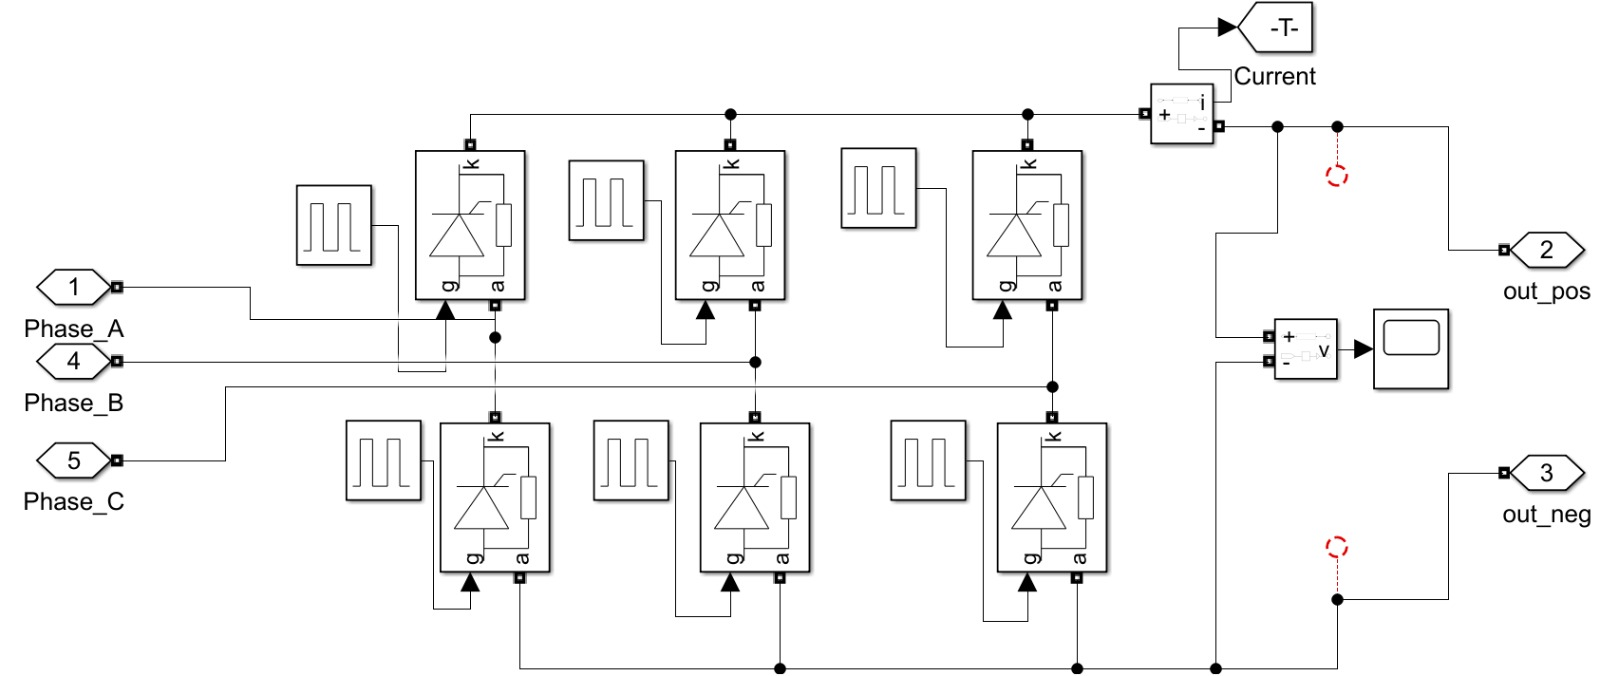
\includegraphics[width=0.5\textwidth]{images/three_phase_rectifier.jpeg}
    \caption{Rectifier Circuit}
    \label{rectifier_circuit}
\end{figure}

After the converting AC to DC, we maintain the voltage and current levels for CCCV Mode using Buck converter as shown in fig. \ref{buck_converter}.
\begin{figure}[htbp]
    \centering
    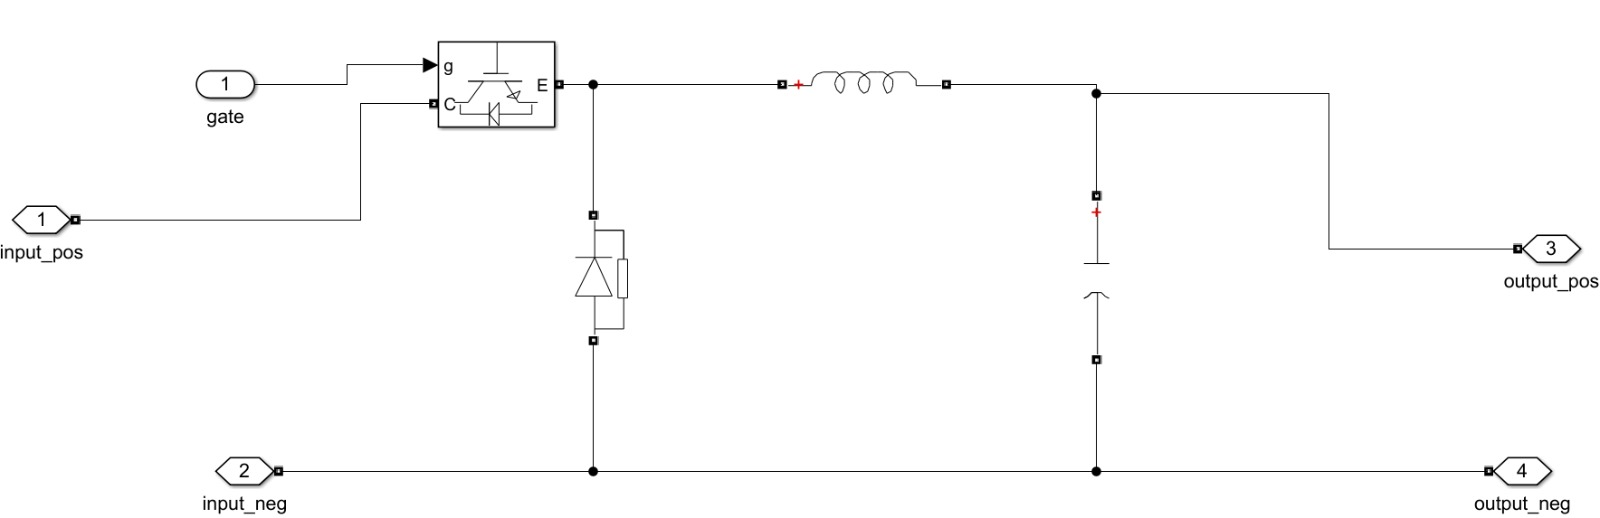
\includegraphics[width=0.5\textwidth]{images/buck_converter.jpeg}
    \caption{Buck Converter}
    \label{buck_converter}
\end{figure}

And for controlling the voltage and current, we are using feedback as shown in fig. \ref{control} and \ref{feedback}.
\begin{figure}[htbp]
    \centering
    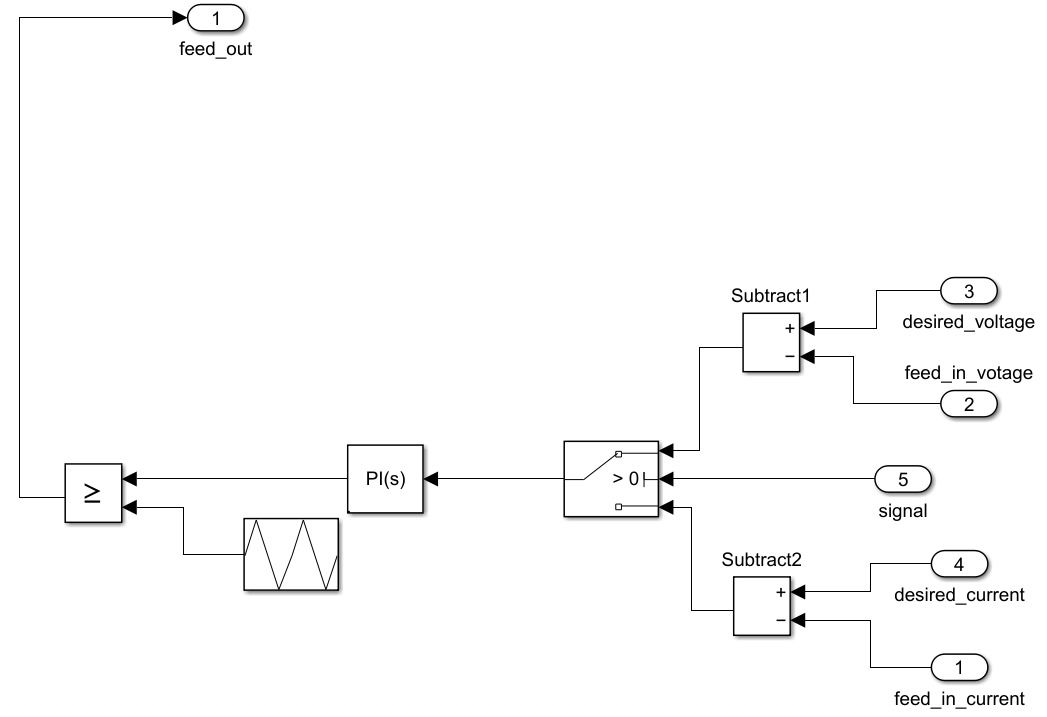
\includegraphics[width=0.5\textwidth]{images/feedback.jpeg}
    \caption{Feedback}
    \label{feedback}
\end{figure}

\begin{figure}[htbp]
    \centering
    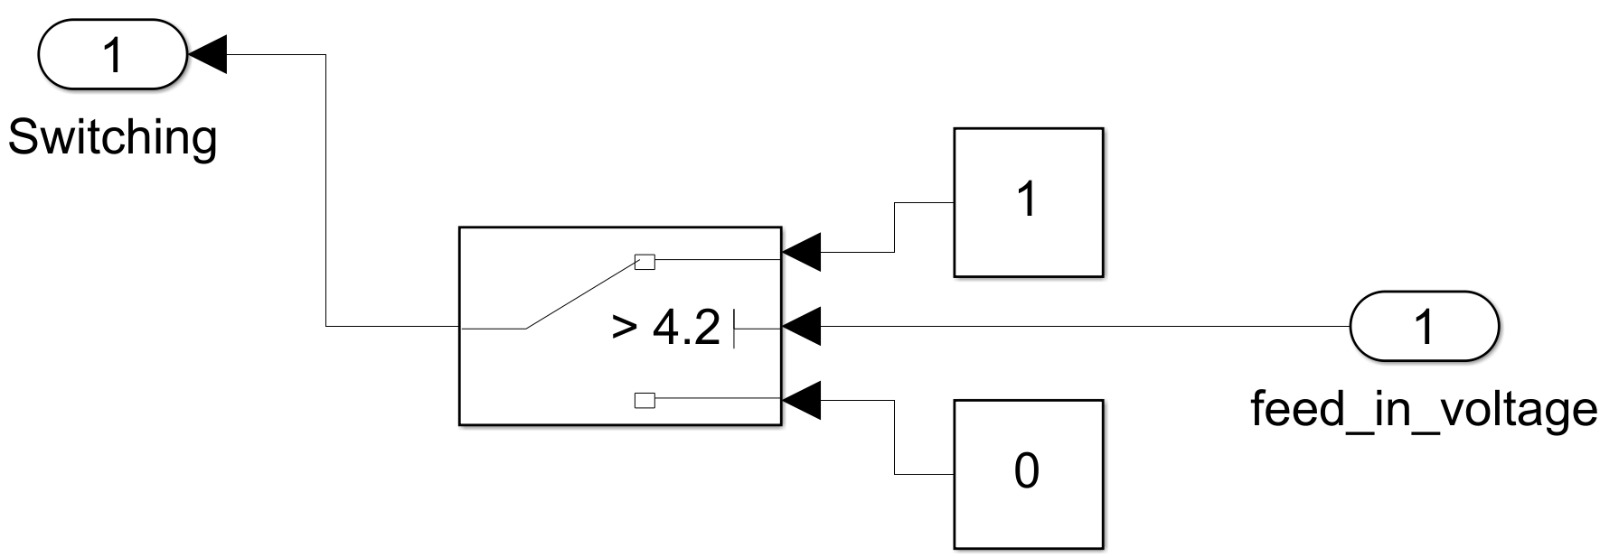
\includegraphics[width=0.5\textwidth]{images/control.jpeg}
    \caption{Control}
    \label{control}
\end{figure}

\subsection{Estimated Kalman Filter :}
The EKF SOC Estimation function, implementing a second-order RC equivalent circuit model (ECM) and extended Kalman Filter (EKF) or adaptive-extended Kalman Filter (AEKF), is a critical tool for estimating a battery's terminal voltage (Vt) and state of charge (SOC). This function relies on publicly available battery datasets for calibration and validation, including the Turnigy Graphene 5000mAh 65C Li-ion Battery Data, LG 18650HG2 Li-ion Battery Data, Panasonic 18650PF Li-ion Battery Data, and Samsung INR21700 30T 3Ah Li-ion Battery Data \cite{turnigy_data}\cite{lg_data}\cite{samsung_data}\cite{panasonic_data}.


\subsubsection{Initialization:}
\begin{itemize}
  \item Load battery parameters and SOC-OCV relationships from provided data files.
  \item Initialize battery model parameters and SOC-OCV curve.
  \item Set initial SOC, state space parameters, and sample time.
  \item Consider the ECM with equation.
  $${V_t = V_{OC} - V_1 - V_2}$$
  where $V_t$ is the terminal voltage of the battery, $V_{OC}$ is the OCV of the battery, $V_1 \& V_2$ is the voltage across parallel $R_1, C_1 and R_2, C_2$.
\end{itemize}

\subsubsection{Model Initialization:}
\begin{itemize}
  \item Initialize scatteredInterpolant functions for battery parameters and SOC-OCV curve.
  \item Fit an odd-order polynomial to the SOC-OCV data.
\end{itemize}

\subsubsection{Kalman Filter Parameters Initialization:}
\begin{itemize}
  \item Set initial values for Kalman Filter parameters.
  \item Adjust parameters manually or through optimization algorithms for specific batteries and drive cycles.
\end{itemize}

\subsubsection{Loop Execution:}
\begin{itemize}
  \item Iterate through the length of the input current vector.
  \item Evaluate battery parameters for the current temperature and SOC.
  \item Calculate A and B matrices for the ECM.
  \[ A = 
\begin{bmatrix}
    1 & 0 & 0 \\
    0 & exp^{\frac{-\Delta t}{R_1C_1}} & 0 \\
    0 & 0 & exp^{\frac{-\Delta t}{R_2C_2}}
\end{bmatrix}
\]

\[ B = 
\begin{bmatrix}
    -\frac{\delta t}{Q}\eta[k]\\
    R_1(1-exp^{\frac{-\Delta t}{R_1C_1}}) \\
    R_2(1-exp^{\frac{-\Delta t}{R_2C_2}})
\end{bmatrix}
\]
  \item Run the update model to compute terminal voltage.
  \item Linearize the model and calculate Vt error.
\end{itemize}

\subsubsection{EKF Execution:}
\begin{itemize}
  \item Perform the prediction (time update) step of the EKF.
  \item Project the states ahead and update error covariance.
  $${\hat{x}_{k+1|k} = A\hat{x}_{k|k} + B_{u_k}}$$
  $${\hat{P}_{k+1|k} = A\hat{P}_{k|k}A^T + Q_{k}}$$
  \item Perform the correction (measurement update) step of the EKF.
  \item Compute Kalman gain, update estimate with measurement $z_k$(a-posteriori), and update error covariance.
  $${K_{k+1} = P_{k+1|k}C_T(CP_{k+1|k}C^T+R_{k+1})^{-1}}$$
  $${\hat{x}_{k+1|k+1} = \hat{x}_{k+1|k} + K_{k+1}(z_{k+1} - C\hat{x}_{k+1|k})}$$
  $${\hat{P}_{k+1|k+1} = (1-K_{k+1}C)\hat{P}_{k+1|k} }$$
\end{itemize}


\subsubsection{Output:}
\begin{itemize}
  \item Store the estimated SOC, Vt, and Vt error in output vectors.
\end{itemize}

This function facilitates accurate estimation of battery SOC and terminal voltage, crucial for battery management in various applications. Tuning of Kalman Filter parameters and careful initialization of battery model parameters ensure reliable performance across different battery types and operating conditions.\newline
\textbf{Note :} The code of the Extended Kalman Filter can be found in my GitHub Repository \cite{github_repo}.

\section{Observation :}
\subsection{Battery Charging Mode Shift}
\hspace{0.5cm}The fig. \ref{battery_parameters} shows the current, voltage and state of charge of battery in simulink with respect to the battery.\newline
\begin{figure}[htbp]
    \centering
    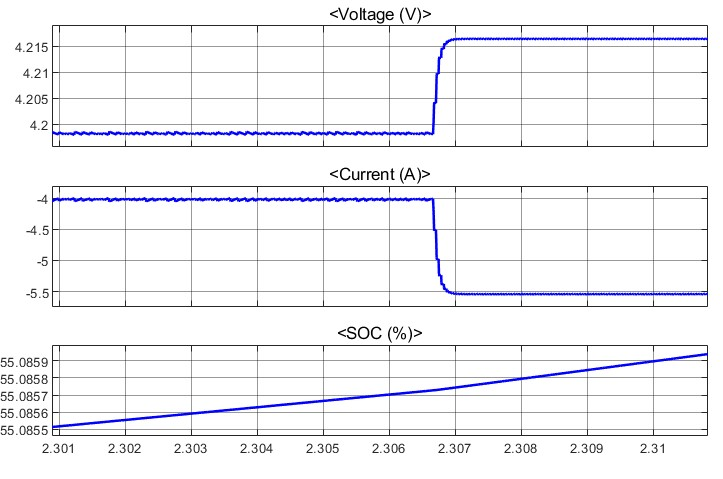
\includegraphics[width=0.5\textwidth]{images/battery_params.jpeg}
    \caption{Battery Parameters}
    \label{battery_parameters}
\end{figure}
\hspace{0.5cm} It can be observed that the charging mode is changing from constant current and constant voltage at around time t = 2.3065s. The measurement reading with respect to measurement sensors is given in fig. \ref{measurement_block}, here too it can be observed that there is a change in charging mode.
\begin{figure}[htbp]
    \centering
    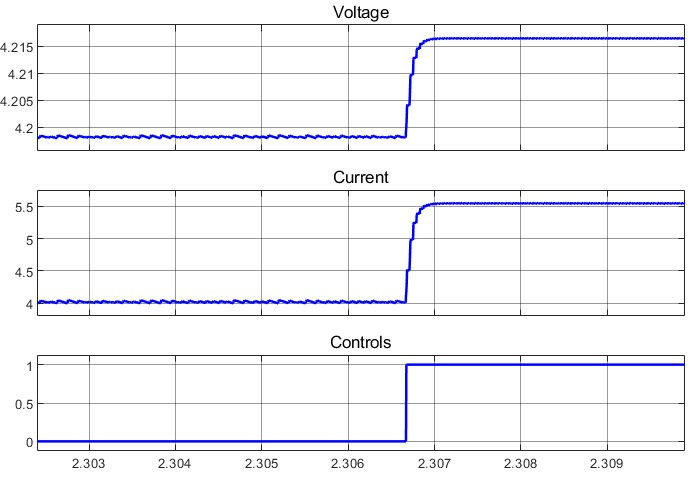
\includegraphics[width=0.45\textwidth]{images/measurement_block.jpeg}
    \caption{Measurements}
    \label{measurement_block}
\end{figure}
\subsection{SOC estimation}
\hspace{0.5cm}The SOC estimation for battery in this case Turnigy Graphene 5000mAh 65C Li-ion Battery is done, by discharging the battery from 100\% is shown in fig. \ref{soc_estimation_curve}.
\begin{figure}[htbp]
    \centering
    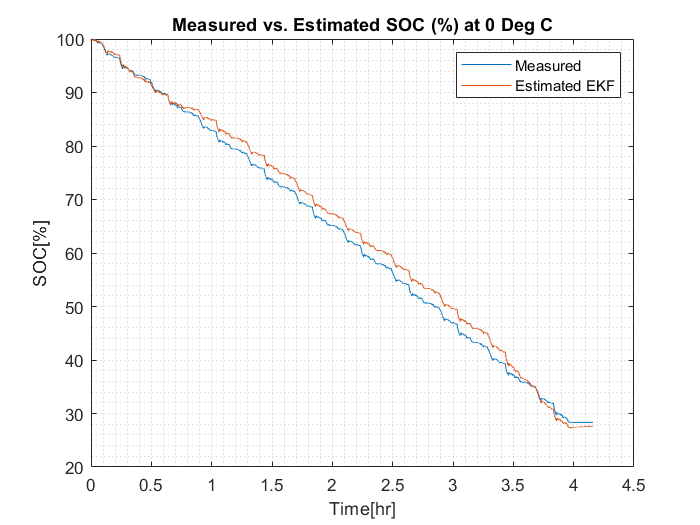
\includegraphics[width=0.45\textwidth]{images/soc_estimation_curve.png}
    \caption{SOC Estimation Curve}
    \label{soc_estimation_curve}
\end{figure}
\begin{figure}[htbp]
    \centering
    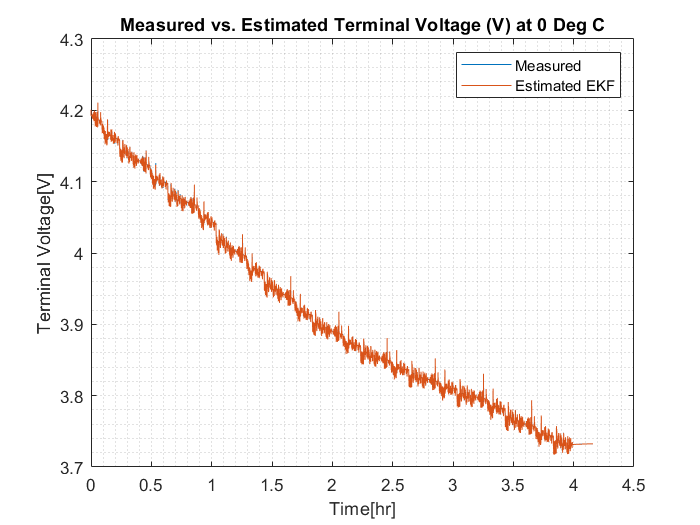
\includegraphics[width=0.45\textwidth]{images/voltage_estimation_curve.png}
    \caption{Voltage Estimation Curve}
    \label{voltage_estimation_curve}
\end{figure}
\newline The error in estimated and measured voltage is almost negligible as seen in fig. \ref{voltage_estimation_curve}, the estimated and measurement voltage are almost overlapping.
\begin{figure}[htbp]
    \centering
    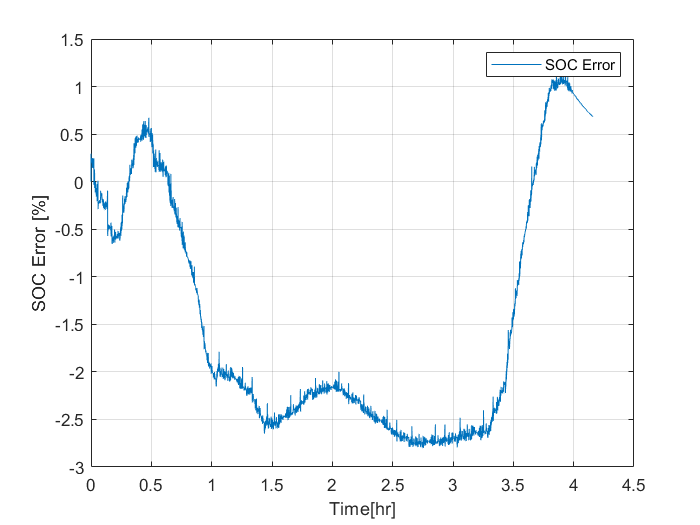
\includegraphics[width=0.5\textwidth]{images/soc_error.png}
    \caption{SOC Error}
    \label{soc_error}
\end{figure}
\newline
Consider fig. \ref{soc_error}, showing the error in SOC. This curve shows the variation of accuracy in SOC which can be obtained in any cell with its particular battery data.

\section{Result :}
\section{Conclusion and Future Scope :}
The simulation phase of the on-board electrical vehicle charger employing the CCCV charging method marks a significant milestone in our major project. Through MATLAB simulation, we have meticulously analyzed and optimized the charging system, incorporating components like the Buck Converter and 3-phase rectifier. This simulation work provides crucial insights into the charging efficiency, current control, and voltage regulation, laying a strong foundation for the subsequent practical implementation. The SOC estimation through Extended Kalman filter was achieved successfully.

In future endeavors, our focus lies in advancing the current charging system. Key initiatives include developing a cutting-edge battery with integrated State of Charge (SOC) monitoring for real-time updates on energy levels. Additionally, there's a need to work on making hardware, transitioning from simulation to practical implementation. The vision extends to an intelligent Battery Management System (BMS) capable of adaptive charging strategies based on real-time SOC data, deploying algorithms for optimal energy use. Exploring advanced control strategies seeks to optimize the buck converter’s efficiency during Constant Current Constant Voltage (CCCV) charging. Overall, our goal is to not only refine the existing system but also contribute to the evolution of battery technology and intelligent charging infrastructure.

\begin{thebibliography}{00}
\bibitem{github_repo} electrical\_vehicle\_battery\_charger GitHub Repository. (n.d.). Retrieved from \url{https://github.com/SanketSarmalkar/electrical_vehicle_battery_charger}

\bibitem{turnigy_data} Turnigy Graphene 5000mAh 65C Li-ion Battery Data. Available at: \url{https://data.mendeley.com/datasets/4fx8cjprxm/1}

\bibitem{lg_data} LG 18650HG2 Li-ion Battery Data. Available at: \url{https://data.mendeley.com/datasets/cp3473x7xv/3}

\bibitem{panasonic_data} Panasonic 18650PF Li-ion Battery Data. Available at: \url{https://data.mendeley.com/datasets/wykht8y7tg/1}

\bibitem{samsung_data} Samsung INR21700 30T 3Ah Li-ion Battery Data. Available at: \url{https://data.mendeley.com/datasets/9xyvy2njj3/1}

\end{thebibliography}
\vspace{12pt}

\end{document}
